\documentclass[11pt]{article}
\usepackage[utf8]{inputenc}
\usepackage{amsmath, amssymb, amsthm}
\usepackage{graphicx}
\usepackage{geometry}
\usepackage{tikz}
\usepackage{float}
\usepackage{caption}
\usepackage{hyperref}
\usepackage{authblk} 

\usetikzlibrary{arrows.meta, decorations.markings, calc, patterns, shapes.geometric}
\geometry{margin=1in}

\title{Hyperbolic Modeling of Reputation: Karma as a Poincar\'e Disk Fiber Bundle}
\author[1]{Ismael S. Silva}
\affil[1]{Universidade Federal do Cear\'a\\ \texttt{ismaelsoares.pro@alu.ufc.br}}
\date{}

\begin{document}

\maketitle

\noindent\textbf{Keywords:} reputation, hyperbolic geometry, multi-agent systems, trust modeling, Poincar\'e disk

\begin{abstract}
We propose a novel model of social reputation---referred to as "karma"---based on hyperbolic geometry. Specifically, we represent an agent's moral or reputational state as a point on the Poincar\'e disk, where the magnitude indicates reputational strength and the angular coordinate encodes moral orientation. To incorporate context-dependence, we construct a fiber bundle over the disk, associating each point with a contextual space (e.g., professional, personal). The hyperbolic metric naturally models the sensitivity of high-reputation agents to minor transgressions and allows for counterintuitive proximities between morally opposite individuals. We formalize karma dynamics as a stochastic differential equation on the hyperbolic space. This geometric approach provides a lightweight, expressive alternative to complex probabilistic models, with potential applications in multi-agent reinforcement learning, social simulations, and ethical AI systems.
\end{abstract}

\section{Introduction}
Reputation systems are central to agent interaction in multi-agent environments, social simulations, and ethical modeling. Traditional approaches, such as scalar scores or graph-theoretic trust networks \cite{sabater2005review, josang2002subjective}, often fail to capture nuanced phenomena such as:

\begin{itemize}
    \item \textbf{Moral vulnerability of the virtuous}: Small transgressions have disproportionate effects on individuals with high reputation.
    \item \textbf{Paradoxical trust}: Strongly altruistic agents may express unexpected affinity or trust toward agents with negative reputations.
    \item \textbf{Contextual incommensurability}: Agents with similar aggregate reputations may not trust each other due to differences in context (e.g., personal vs. professional).
\end{itemize}

To address these challenges, we introduce a geometric model of karma using the Poincar\'e disk, inspired by recent successes of hyperbolic embeddings in machine learning \cite{nickel2017poincare}, and a fiber structure to incorporate context. This yields a rich but computationally tractable framework.

\section{Geometric Karma Model}

\subsection{State Space: The Poincar\'e Disk}
The agent's karma is modeled as a point $K$ in the open unit disk $\mathbb{D} = \{ z \in \mathbb{C} : |z| < 1 \}$.
\begin{itemize}
\item $|z|$ measures reputation magnitude.
\item $\arg(z)$ encodes moral orientation.
\item $z=0$ corresponds to a neutral state.
\end{itemize}

The distance between two karma states $z_1$ and $z_2$ is the hyperbolic distance in the Poincar\'e disk model:
\begin{equation}
d_H(z_1, z_2) = \operatorname{arcosh} \left( 1 + \frac{2|z_1 - z_2|^2}{(1 - |z_1|^2)(1 - |z_2|^2)} \right)
\label{eq:hyperbolic_distance}
\end{equation}
This metric amplifies small Euclidean displacements near the boundary ($|z| \to 1$), as illustrated in Figure~\ref{fig:metric_distortion}. This naturally models the instability of high karma values.


\begin{figure}[htbp]
\centering
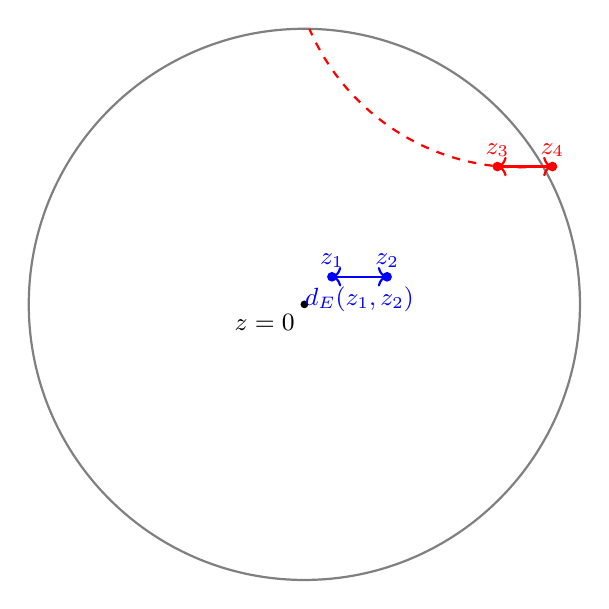
\begin{tikzpicture}[scale=3.5, font=\small]
\draw[thick, gray] (0,0) circle (1);
\node[below left] at (0,0) {$z=0$};
\fill (0,0) circle (0.4pt);
\coordinate (A1) at (0.1, 0.1);
\coordinate (A2) at (0.3, 0.1);
\fill[blue] (A1) circle (0.5pt) node[above] {$z_1$};
\fill[blue] (A2) circle (0.5pt) node[above] {$z_2$};
\draw[<->, blue, thick] (A1) -- (A2) node[midway, below] {$d_E(z_1,z_2)$};
\coordinate (B1) at (0.7, 0.5);
\coordinate (B2) at (0.9, 0.5);
\fill[red] (B1) circle (0.5pt) node[above] {$z_3$};
\fill[red] (B2) circle (0.5pt) node[above] {$z_4$};
\draw[<->, red, thick] (B1) -- (B2);
\begin{scope}
\clip (0,0) circle (1);
\draw[red, thick, dashed] (0.783,1.33) circle (0.833);
\end{scope}
\end{tikzpicture}
\caption{\textbf{Hyperbolic Metric Distortion.} Equal Euclidean distances result in different hyperbolic distances. Near the boundary, hyperbolic distances (dashed red line) grow sharply compared to distances near the center (solid blue line), modeling the reputational instability of agents with extreme karma.}
\label{fig:metric_distortion}
\end{figure}

\subsection{Fiber Structure: Modeling Context}
To account for context, we model the full reputation state as a fiber bundle over the karma disk $\mathbb{D}$. Each point $z \in \mathbb{D}$ (the base space) is associated with a context-specific fiber $F_z$. The total reputation state is a pair $(z, v)$ where $v \in F_z$. This structure is visualized in Figure~\ref{fig:fiber_structure}.


\begin{figure}[htbp]
\centering
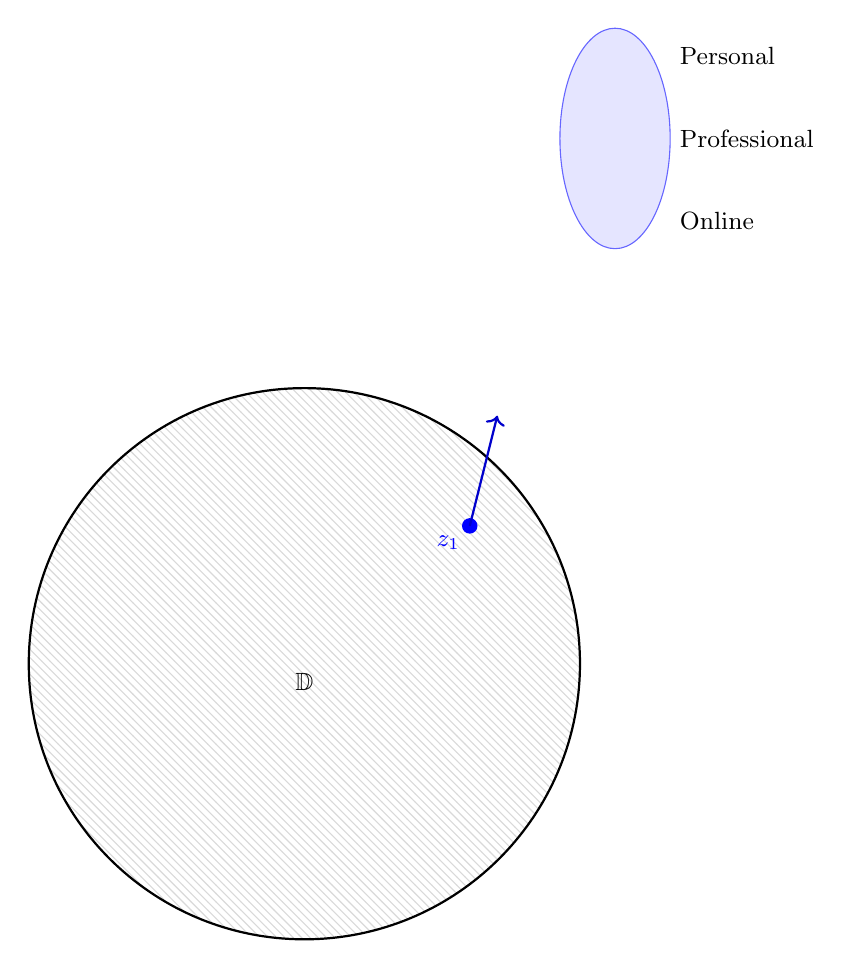
\begin{tikzpicture}[scale=3.5, font=\small]
    \draw[thick, pattern=north west lines, pattern color=gray!30] (0,0) circle (1);
        \node[below] at (0,0) {$\mathbb{D}$};
        \coordinate (z1) at (0.6, 0.5);
        \fill[blue] (z1) circle (0.8pt) node[below left] {$z_1$};
    \draw[->, thick, blue!80!black] (z1) -- ++(0.1, 0.4);
    \begin{scope}[shift={(z1)}, xshift=15, yshift=40]
        \draw[blue!60, fill=blue!10] (0,0) ellipse (0.2 and 0.4);
        \node[right] at (0.2, 0.3) {Personal};
        \node[right] at (0.2, 0) {Professional};
        \node[right] at (0.2, -0.3) {Online};
    \end{scope}
\end{tikzpicture}
\caption{\textbf{Fiber Structure over the Karma Base Space.} Each karma state $z$ in the base disk $\mathbb{D}$ has an associated contextual fiber $F_z$, which captures domain-specific nuances of reputation.}
\label{fig:fiber_structure}
\end{figure}

\subsection{Karma Dynamics}
The evolution of an agent's karma state $z$ over time is modeled by a stochastic differential equation:
\begin{equation}
    \frac{dz}{dt} = -\nabla_H \Phi(z, v) + \rho \cdot \xi(t)
    \label{eq:karma_dynamics}
\end{equation}
where:
\begin{itemize}
    \item $\Phi(z, v)$ is a reputational potential field that depends on both the karma state $z$ and its context $v$.
    \item $\nabla_H$ is the gradient that respects the hyperbolic geometry of the space.
    \item $\xi(t)$ is a stochastic noise term representing random events (e.g., scandals, misinformation), scaled by a factor $\rho$.
\end{itemize}
This formalism allows for complex behaviors, such as the paradoxical trust shown in Figure~\ref{fig:geodesics}, where morally opposite agents might find themselves "close" along a shared hyperbolic geodesic.


\begin{figure}[htbp]
\centering
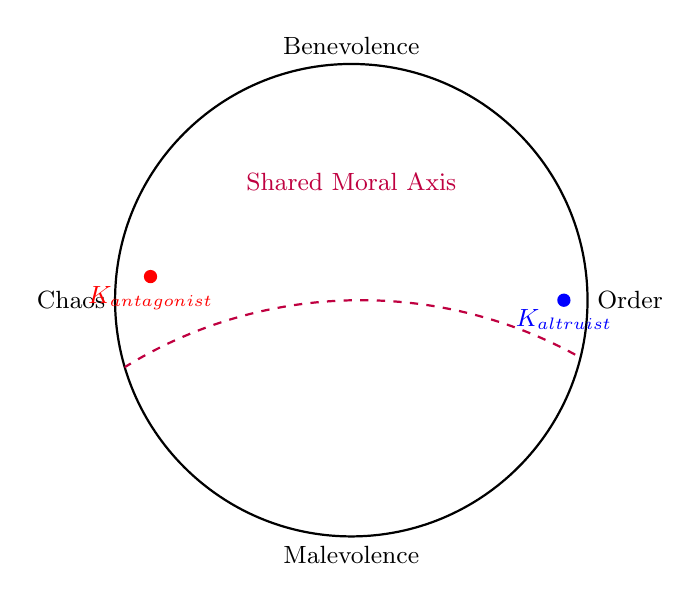
\begin{tikzpicture}[scale=3, font=\small]
    \draw[thick] (0,0) circle (1);
    \node[above] at (0, 1) {Benevolence};
    \node[below] at (0, -1) {Malevolence};
    \node[left] at (-1, 0) {Chaos};
    \node[right] at (1, 0) {Order};
    \coordinate (A) at (0.9, 0);
    \coordinate (B) at (-0.85, 0.1);
    \fill[blue] (A) circle (0.8pt) node[below] {$K_{altruist}$};
    \fill[red] (B) circle (0.8pt) node[below] {$K_{antagonist}$};
    \begin{scope}
        \clip (0,0) circle (1);
        % This geodesic connects the altruist and antagonist along the "Order-Chaos" axis
        \draw[thick, purple, dashed] (0.04, -1.9) circle (1.9);
    \end{scope}
    \node[purple] at (0, 0.5) {Shared Moral Axis};
\end{tikzpicture}
\caption{\textbf{Geodesics and Moral Extremes.} Even agents with antagonistic reputations (e.g., altruist vs. antagonist) may share an alignment along a hyperbolic geodesic (a "shared moral axis"), enabling paradoxical trust or understanding.}
\label{fig:geodesics}
\end{figure}

\section{Applications and Conclusion}
This hyperbolic model of karma enables new forms of analysis and application:
\begin{itemize}
    \item Reputation-aware policy learning in multi-agent reinforcement learning (MARL).
    \item Rich visualization of social and moral dynamics in simulations.
    \item Integration with procedural content generation to create ethically responsive environments.
    \item Simulation of complex social phenomena like ethical drift, moral injury, and reputational recovery.
\end{itemize}

Its key strength lies in using a principled geometric structure to encode complex social phenomena that would otherwise require cumbersome probabilistic machinery. The resulting framework is fast, interpretable, and extensible.


\begin{thebibliography}{9}

\bibitem{sabater2005review}
J. Sabater and C. Sierra, \textit{Review on Computational Trust and Reputation Models}, Artificial Intelligence Review, 2005.

\bibitem{josang2002subjective}
A. J\o sang and R. Ismail, \textit{The Beta Reputation System}, Proceedings of the 15th Bled Electronic Commerce Conference, 2002.

\bibitem{nickel2017poincare}
M. Nickel and D. Kiela, \textit{Poincar\'e Embeddings for Learning Hierarchical Representations}, Advances in Neural Information Processing Systems (NeurIPS), 2017.

\end{thebibliography}

\end{document}